\documentclass[conference]{IEEEtran}

\usepackage{url}
\usepackage{graphicx}
\usepackage{caption}
%\usepackage{subcaption}
\usepackage{subfigure}
\usepackage{hyperref}
\usepackage{url}
\usepackage{times}
\usepackage{balance}
\usepackage{xspace}
\usepackage{paralist}
\usepackage{color}
\usepackage{amssymb}

\clubpenalty = 10000
\widowpenalty = 10000
\displaywidowpenalty = 10000

\begin{document}

\newcommand{\ghtorrent}{\textsc{ght}orrent\xspace}
\newcommand{\prioritizer}{\textsc{pr}ioritizer\xspace}
\newcommand{\api}{\textsc{api}\xspace}
\newcommand{\todo}[1]{\textcolor{red}{\textbf{\textsc{todo:}} #1}}

\newcommand{\nb}[3]{
  \fcolorbox{black}{#2}{\bfseries\sffamily\scriptsize#1}
    {\sf\small$\blacktriangleright$\textit{#3}$\blacktriangleleft$}
}

\newcommand\georgios[1]{\nb{Georgios}{yellow}{#1}}
\newcommand\andy[1]{\nb{Andy}{cyan}{#1}}
\newcommand\erik[1]{\nb{Erik}{magenta}{#1}}

\newcommand{\hassanbox}[1]
{
  \vspace{0.29em}
  \noindent
  \fbox{
  \begin{minipage}{0.46\textwidth}
    \emph{\noindent #1}
    \end{minipage}
}}

% Macros for qualitative research :-)
\newcommand{\resp}[2]{{\sc R#1:} ``\emph{#2}''}
\newcommand{\respnum}[1]{{\sc R#1}}
\newcommand{\code}[1]{{\textsl{#1}}}

%\title{Pull Request Prioritization}
\title{Automatically Prioritizing Pull Requests}


\author{\IEEEauthorblockN{Erik van der Veen}
\IEEEauthorblockA{Delft University of Technology\\
the Netherlands\\
Email: e.v.d.veen@tudelft.nl}
\and
\IEEEauthorblockN{Georgios Gousios}
\IEEEauthorblockA{Radboud University Nijmegen\\
the Netherlands\\
Email: g.gousios@cs.ru.nl}
\and
\IEEEauthorblockN{Andy Zaidman}
\IEEEauthorblockA{Delft University of Technology\\
the Netherlands\\
Email: a.e.zaidman@tudelft.nl}}

\maketitle

\begin{abstract}

In previous work, we observed that in the pull-based development model integrators face challenges with regard to prioritizing work in the face of multiple concurrent pull requests. We present the design and initial implementation of a prototype pull request prioritisation tool called \prioritizer. \prioritizer works like a priority inbox for pull requests, recommending the top pull requests the project owner should focus on. A preliminary user study showed that \prioritizer provides functionality that GitHub is currently lacking, even though users needed more insight into how the priority ranking is established to make \prioritizer really useful.

\end{abstract}

%\category{D.2.7}{Software Engineering}{Distribution, Maintenance, and Enhancement}[Version control]
%\category{D.2.9}{Software Engineering}{Management}[Programming teams]

%\terms{Management}

%\keywords{pull-based development, pull request, distributed software development,
%empirical software engineering}

\section{Introduction}

Pull-based development as a distributed development model is a distinct way of
collaborating in software development. In this model, the project's main
repository is not shared among potential contributors; instead, contributors
fork (clone) the repository and make their changes independent of each other.
When a set of changes is ready to be submitted to the main repository, they
create a pull request, which specifies a local branch to be merged with a branch
in the main repository. A member of the project's core team (the
\emph{integrator}) is responsible to inspect the changes and integrate them into
the project's main development line.

In earlier work~\cite{GZSD15}, we surveyed 750 pull request integrators from high
volume projects and discovered that the top two challenges they face when
working with pull requests are maintaining project quality and prioritizing work
in the face of multiple concurrent pull requests. With respect to pull request
prioritization our findings are summarized in Figure~\ref{fig:prioritization}.

In this paper, we present the design and initial implementation of a prototype
pull request prioritization tool, the \prioritizer. \prioritizer works as a
priority inbox for pull requests: it examines all open pull requests and
presents project integrators the top pull requests that potentially need their immediate
attention. It also offers an alternative view to Github's pull request
interface, which allows developers to sort open pull requests on a multitude of
criteria, ranging from the pull request's age to its number of conflicts with
other open pull requests (pairwise conflicts). \prioritizer is a service-oriented architecture build on top of
\ghtorrent~\cite{G13}: it uses \ghtorrent's data collection mechanisms to react in near real-time to changes in pull request state.


\begin{figure}[t]
  \begin{center}
    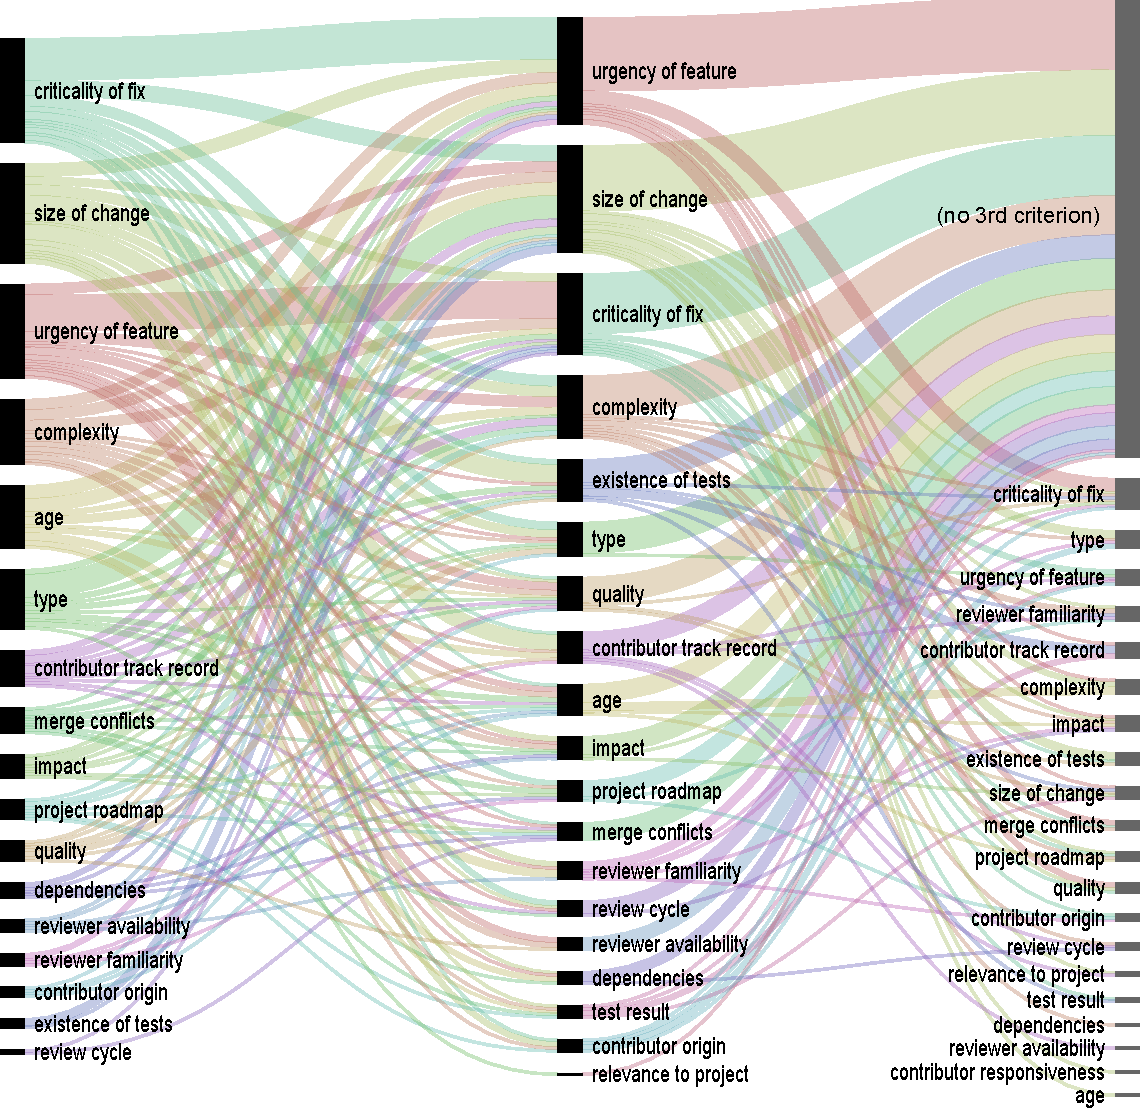
\includegraphics[scale=0.44]{../figs/prioritization-criteria}
  \end{center}
  \caption{Prioritization criteria and their order of application as reported by
  750 integrators~\cite{GZSD15}.}
  \label{fig:prioritization}
\end{figure}


\section{Prioritizing pull requests}

\subsection{Modeling} 
Contrary to work prioritization approaches that support development-oriented 
decisions (e.g. bug triaging)~\cite{AnvikTSE2011,Jeong:2009:IBT:1595696.1595715,Tamrawi:2011:FSC:2025113.2025163}, we modelled the pull 
request prioritization using the priority inbox approach~\cite{Conway2011}. The
difference lies in that we do not only look at static information with regard to the 
pull requests, but we also take into account previous actions on pull requests. 
What \prioritizer tries to do is present the integrators with the pull requests 
that will need their immediate attention.

To select the important pull requests, \prioritizer uses machine learning.
Initially, time is split in configurable time windows (currently, 1 day long).
In each time window, \prioritizer calculates a list of features for all pull
requests (dependent variables, explained below) and a boolean response variable
that indicates whether the pull request received a user action in the following
time window. A machine learning algorithm is then trained on historical data to
build a model for predicting whether current pull requests will receive user
updates in the following time window. The pull requests with the highest
probability to be updated are classified as the important ones.

\subsection{Features}
\label{sec:features}
Our feature set was extracted by analysing the results of the
survey~\cite{GZSD15} and closely correspond to the developer's answers as
reported in Figure~\ref{fig:prioritization}. An overview of the selected
features can be seen in Table~\ref{tab:features}.

\begin{table*}[ht]
  \centering
  \begin{tabular}{rp{26em}rrrrc}
    \hline
    \textbf{Feature} & \textbf{Description} & \textbf{5\%} & \textbf{Mean} & \textbf{Median} & \textbf{95\%} & \textbf{Plot} \\
    \hline
    Age & Minutes between open and the current time window start time. & 0.00 & 167344.02 & 77760.00 & 646560.00 & 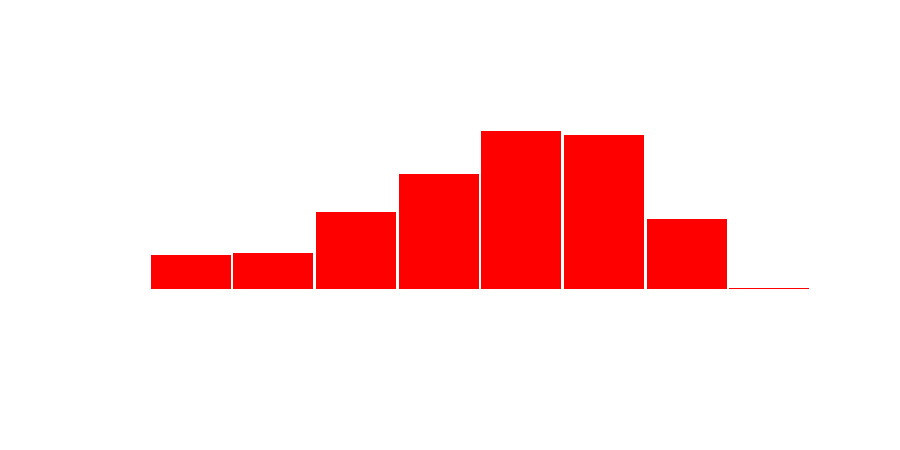
\includegraphics[scale = 0.09, clip = true, trim= 50px 60px 50px 60px]{../figs/hist-features/hist-age.pdf} \\
    Contribution Rate & The percentage of commits by the author currently in the project. & 0.00 & 0.03 & 0.00 & 0.094 & 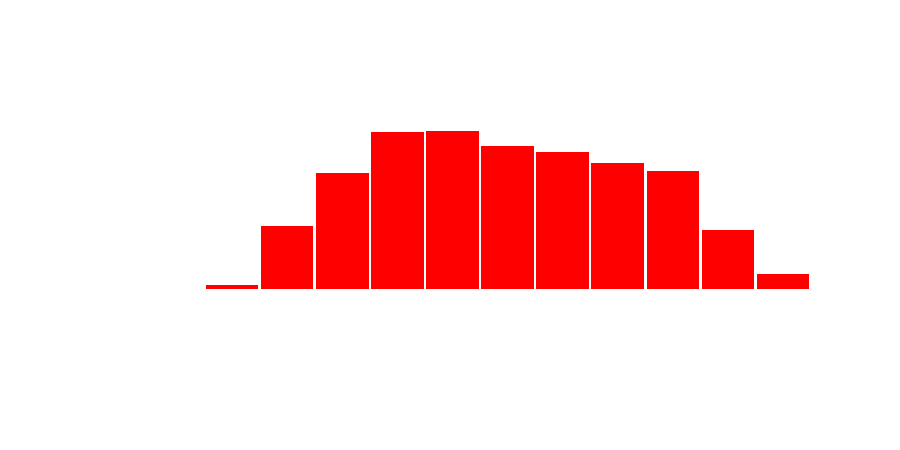
\includegraphics[scale = 0.09, clip = true, trim= 50px 60px 50px 60px]{../figs/hist-features/hist-commitRatio.pdf} \\
    Accept Rate & The percentage of the author's other PRs that have been merged. & 0.00 & 0.45 & 0.50 & 0.90 & 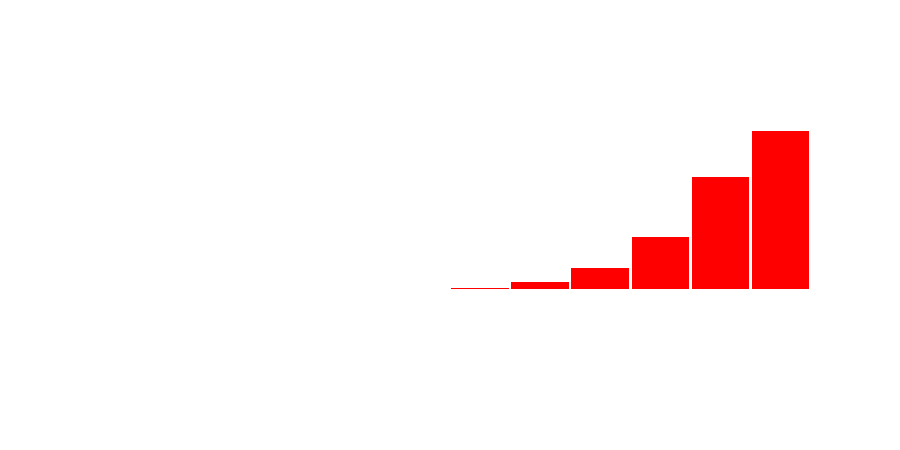
\includegraphics[scale = 0.09, clip = true, trim= 50px 60px 50px 60px]{../figs/hist-features/hist-pullRequestRatio.pdf} \\
    Additions & Number of lines added. & 1.00 & 3649.86 & 41.00 & 6285.00 & 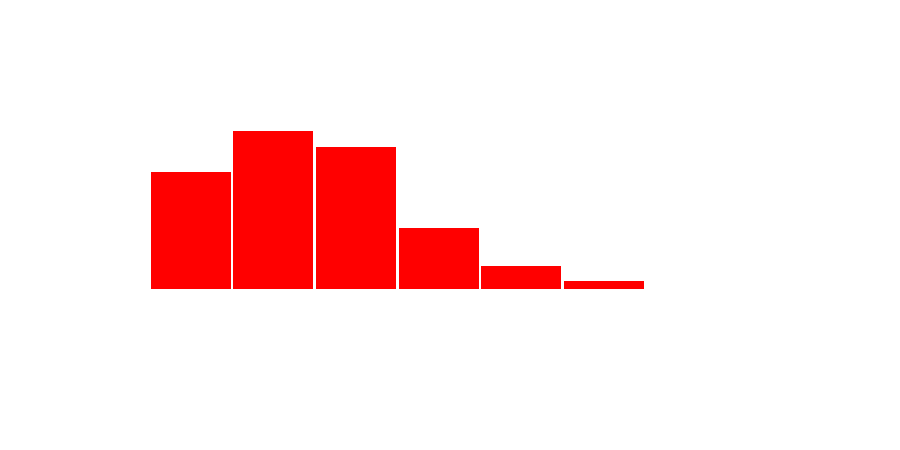
\includegraphics[scale = 0.09, clip = true, trim= 50px 60px 50px 60px]{../figs/hist-features/hist-additions.pdf} \\
    Deletions & Number of lines deleted. & 0.00 & 2271.32 & 7.00 & 2353.00 & 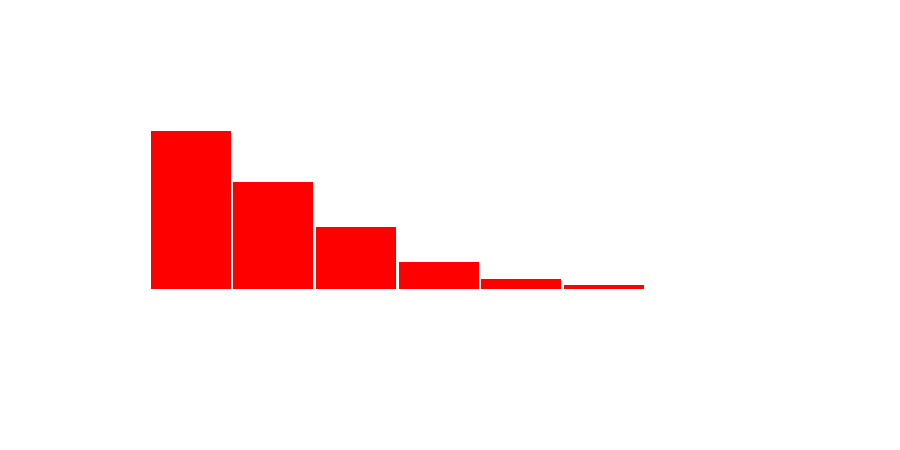
\includegraphics[scale = 0.09, clip = true, trim= 50px 60px 50px 60px]{../figs/hist-features/hist-deletions.pdf} \\
    Commits & Number of commits. & 1.00 & 6.52 & 2.00 & 22.00 & 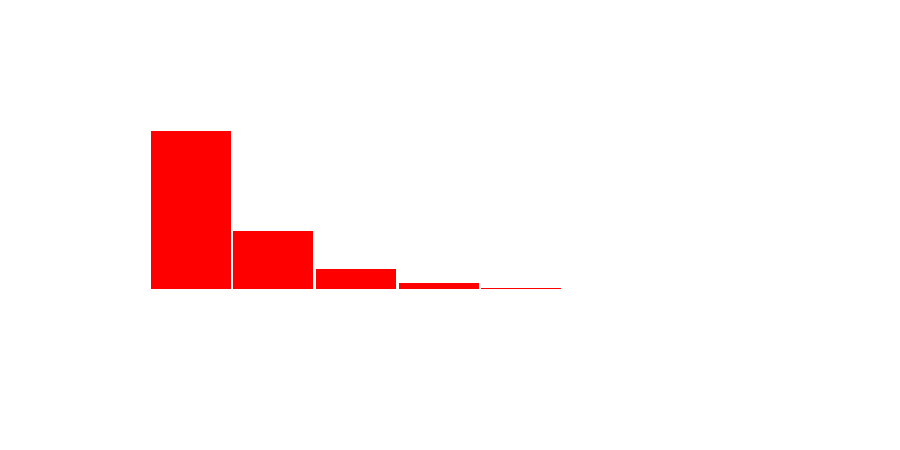
\includegraphics[scale = 0.09, clip = true, trim= 50px 60px 50px 60px]{../figs/hist-features/hist-commits.pdf} \\
    Files & Number of files touched. & 1.00 & 53.88 & 2.00 & 125.00 & 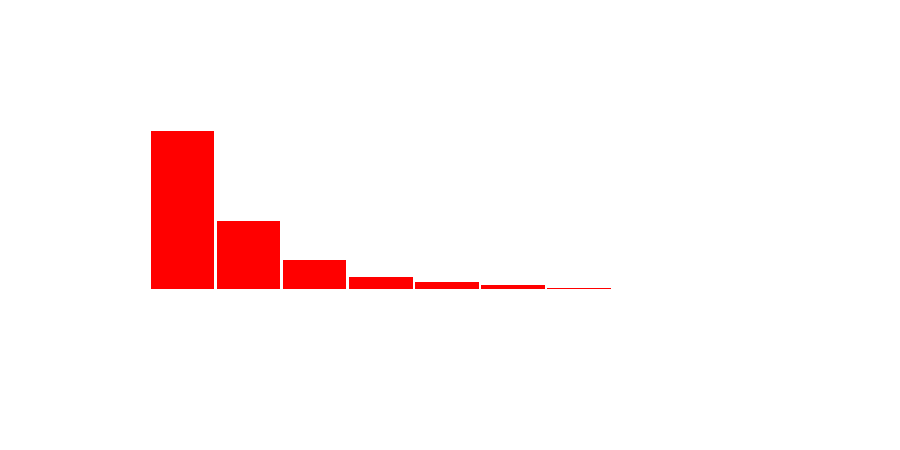
\includegraphics[scale = 0.09, clip = true, trim= 50px 60px 50px 60px]{../figs/hist-features/hist-files.pdf} \\
    Comments & Number of discussion comments. & 0.00 & 4.22 & 1.00 & 17.00 & 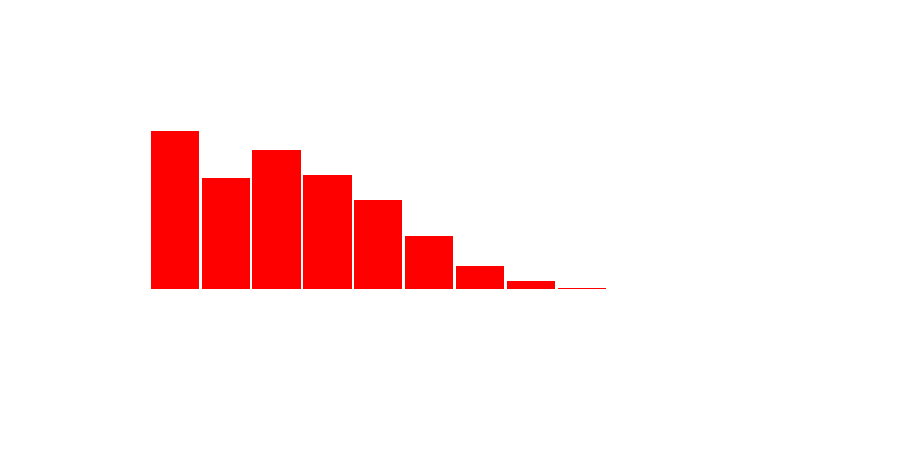
\includegraphics[scale = 0.09, clip = true, trim= 50px 60px 50px 60px]{../figs/hist-features/hist-comments.pdf} \\
    Review Comments & Number of code review comments. & 0.00 & 1.60 & 0.00 & 8.00 & 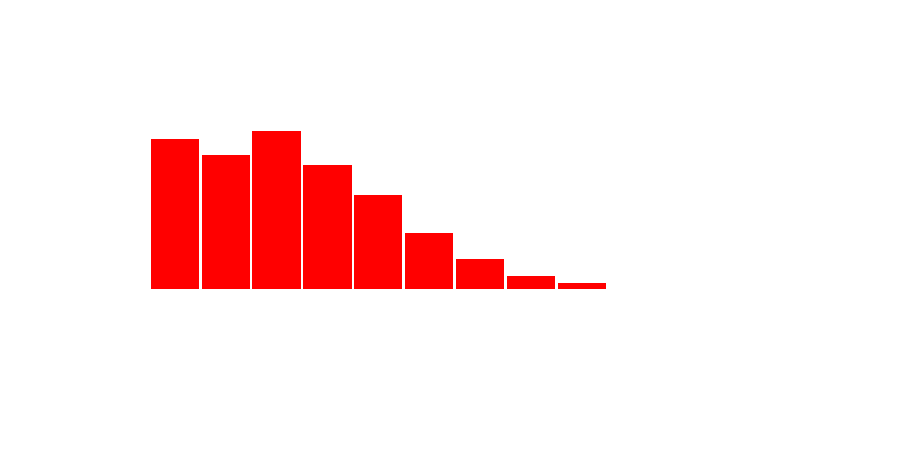
\includegraphics[scale = 0.09, clip = true, trim= 50px 60px 50px 60px]{../figs/hist-features/hist-reviewComments.pdf} \\
    Core Member & Is the author a project member? & 0.00 & 0.26 & 0.00 & 1.00 & 
\includegraphics[scale = 0.09, clip = true, trim= 50px 60px 50px 60px]{../figs/hist-features/hist-coreMember.pdf} \\
    Intra-Branch & Are the source and target repositories the same? & 0.00 & 0.06 & 0.00 & 1.00 & 
\includegraphics[scale = 0.09, clip = true, trim= 50px 60px 50px 60px]{../figs/hist-features/hist-intraBranch.pdf} \\
    Contains Fix & Is the pull request an issue fix? & 0.00 & 0.098 & 0.00 & 1.00 & 
\includegraphics[scale = 0.1, clip = true, trim= 50px 60px 50px 60px]{../figs/hist-features/hist-containsFix.pdf} \\
    Last Comment Mention & Does the last comment contain a user mention? & 0.00 & 0.091 & 0.00 & 1.00 & 
\includegraphics[scale = 0.1, clip = true, trim= 50px 60px 50px 60px]{../figs/hist-features/hist-lastCommentMention.pdf} \\
    Has Test Code & Are tests included? & 0.00 & 0.35 & 0.00 & 1.00 & 
\includegraphics[scale = 0.09, clip = true, trim= 50px 60px 50px 60px]{../figs/hist-features/hist-hasTestCode.pdf} \\
%    Target Branch & The name of the target branch. & - & - & - & - & \\
%    Pairwise Conflicts & The number of pairwise conflicts with other PRs. & - & - & - & - & \\
    \hline
  \end{tabular}
  \caption{Selected features and descriptive statistics for predicting pull
  request activity. The calculation unit is a pull request.
  Histograms (red) are in log scale.}
  \label{tab:features}
\end{table*}

One of the top parameters that developers examine when prioritizing is the
\textsl{size of change}. We therefore include 4 related features in our
model, namely additions, deletions, commits and files.
Developers also deem the \textsl{age} of the pull request important: we measure
it within the examined time window as the elapsed time between the time window
start and the pull request creation.
The \textsl{contributor's track record} is also taken into account by
integrators. To approximate the track record, we use 3 features: whether
contributors are core team members, their contribution rate and their pull
request acceptance rate. The contribution rate is calculated by taking the number of
commits which are authored by the contributor and included in the project
divided by the total number of commits in the project. Finally, a feature that emerges as important second
prioritization criterion is the \textsl{existence of tests}. In some projects it
is often expected that new pull requests contain tests for the code they modify or
add. Tests are identified by simple heuristics: if ``test'' or ``spec'' are in
the file path of any file affected by the pull request, then the pull request
is marked as having tests.

\section{Design and Implementation}
\label{sec:design}

\begin{figure}
  \centering
  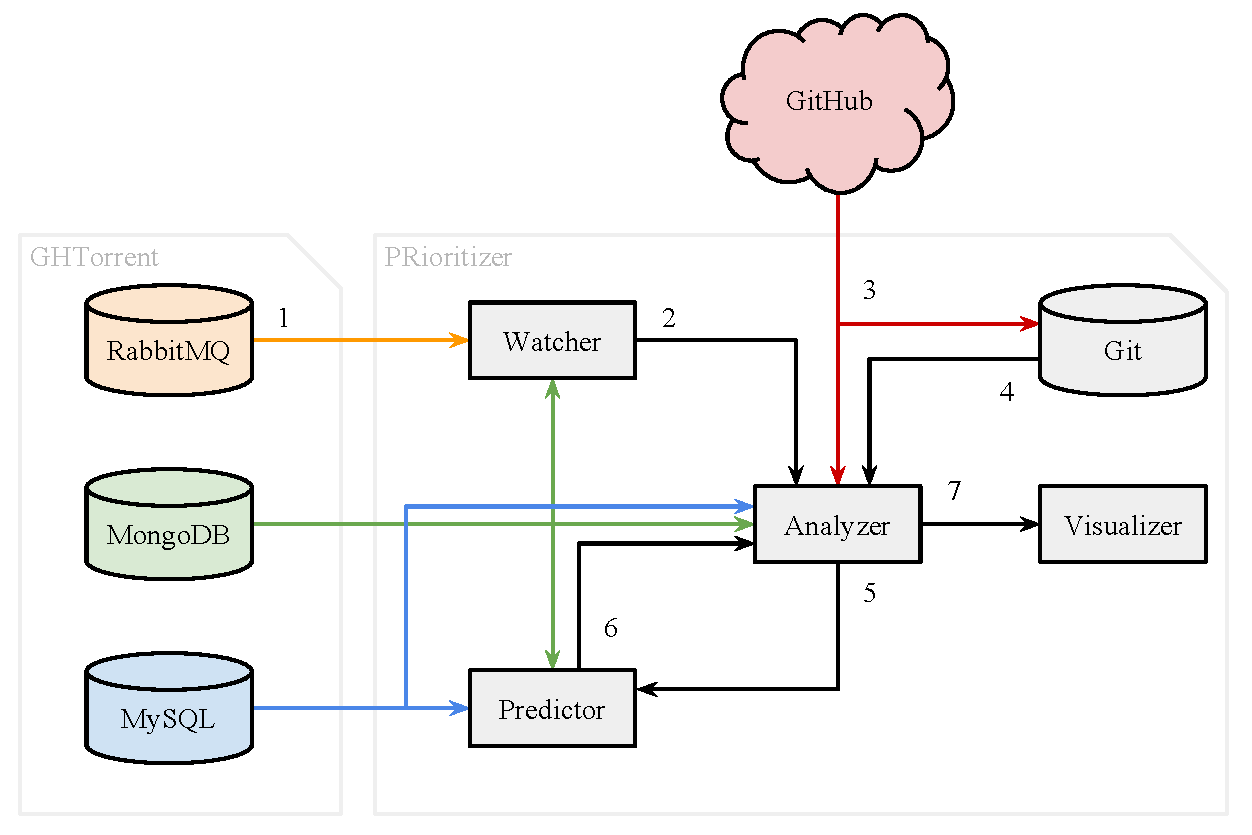
\includegraphics[width=0.5\textwidth]{../figs/architecture.pdf}
  \caption[Diagram of the architecture]
   {Diagram of the architecture. It shows the different data sources and components used by the \prioritizer service.}
  \label{fig:architecture}
\end{figure}

We designed \prioritizer as a loosely-coupled architecture based on independent
micro services. Figure~\ref{fig:architecture} shows a global overview of the
architecture.  The \prioritizer service uses two main data sources: GitHub and
the \ghtorrent project.  When an event arrives the \emph{watcher} component is
notified (1) and starts prioritizing the project (2).  When the \emph{analyzer}
gets a prioritization request, it fetches a list of open pull requests from
GitHub and the pull request contents to the local Git clone (3).  When the data
is fetched, the analyzer processes each pull request in the list with data from the local
clone and \ghtorrent (4).  The data is now ready to be processed by the
\emph{predictor} (5), which generates an ordering for the pull requests.  After
the ordered list is returned to the analyzer (6), the output is generated and
available for the \emph{visualizer} (7).  Details about the design are presented 
in the following sections.

\paragraph{GHTorrent}
\ghtorrent~\cite{G13} mirrors all data exposed from the GitHub \api in
real time. It monitors the GitHub event timeline \api endpoint and publishes the 
retrieved data to a queue service (RabbitMQ) where multiple clients can connect to. 
It also maintains 2 databases, an unstructured one (MongoDB)
which contains the raw replies from the GitHub \api and a relational one
(MySQL) which stores indexed historical data for all GitHub repositories.
\prioritizer uses \ghtorrent as a source for both live and historical data. The live data
that the \prioritizer is interested in are events on pull requests triggered by actions 
such as assignment of the pull request to a specific user or merging the pull request.

\paragraph{Watcher}
The watcher listens to pull request event from \ghtorrent
via a RabbitMQ message queue. It maintains a list of registered repositories
and informs the analyzer when pull request events for one of those is
repositories is received.

\paragraph{Analyzer}
The analyzer analyzes pull request events and computes values for
the features presented in Section~\ref{sec:features}. To do so, for each repository,
it maintains a local Git checkout and a list of open pull requests.
On every pull request event, it updates both the Git repository with
a branch corresponding to the source branch of the pull request
and the open pull request list with fresh information from \ghtorrent.
Then, it uses both \ghtorrent and information into the raw pull request
data to calculate all features in the current time window.

The analyzer also implements a high-performance pull request pairwise conflict
detection mechanism that works by simulating pairwise merges in memory. To avoid
recomputing valid branch merges, it caches intermediate results.

To maintain high performance, all independent processes (Git repository
updating, conflict detection etc) are initiated asynchronously and their
results are gradually composed towards a final set of metrics for the processed
pull request.

\paragraph{Predictor}
The predictor calculates the probability that a specific pull request will
be active within the next time window. To do so, it maintains a per repository
model extracted by applying a machine learning algorithm to existing pull
requests and then uses the computed model to calculate probabilities for
currently updated pull requests.

The predictor is split in two parts: the historic data calculator and
the machine learning implementation. The first shares code (but not the
runtime) with the analyzer as both tools basically compute the same
values in different time windows. To capitalize on the wealth of available
options in statistical environments such as R, the machine learning
part is implemented as a different service that communicates with the
main predictor process through file exchange.

\paragraph{Visualizer}

The visualizer visualizes a list of pull requests, enriched with extra
information extracted from the analysis and prediction phases.  To address
reported deficiencies in GitHub's pull request user interface (also discovered
through our user survey), the visualizer supports filtering pull requests based
on specific branches, originating in specific authors, having conflicts or tests
and being in a mergable state.  It also supports sorting pull requests based on
a multitude of criteria, including all features reported in
Section~\ref{sec:features}.  A key feature of the visualizer is support for user
feedback on the prioritization; the user can report if the proposed
prioritization order is correct and change it to indicate what is the correct
one. At the moment, this information is only collected; in the future, we plan
to use it in order to improve the prioritization algorithm.

The visualizer is implemented as a static web application; a
screenshot of its main page can be seen in Figure~\ref{fig:ui}.

\begin{figure}
  \centering
  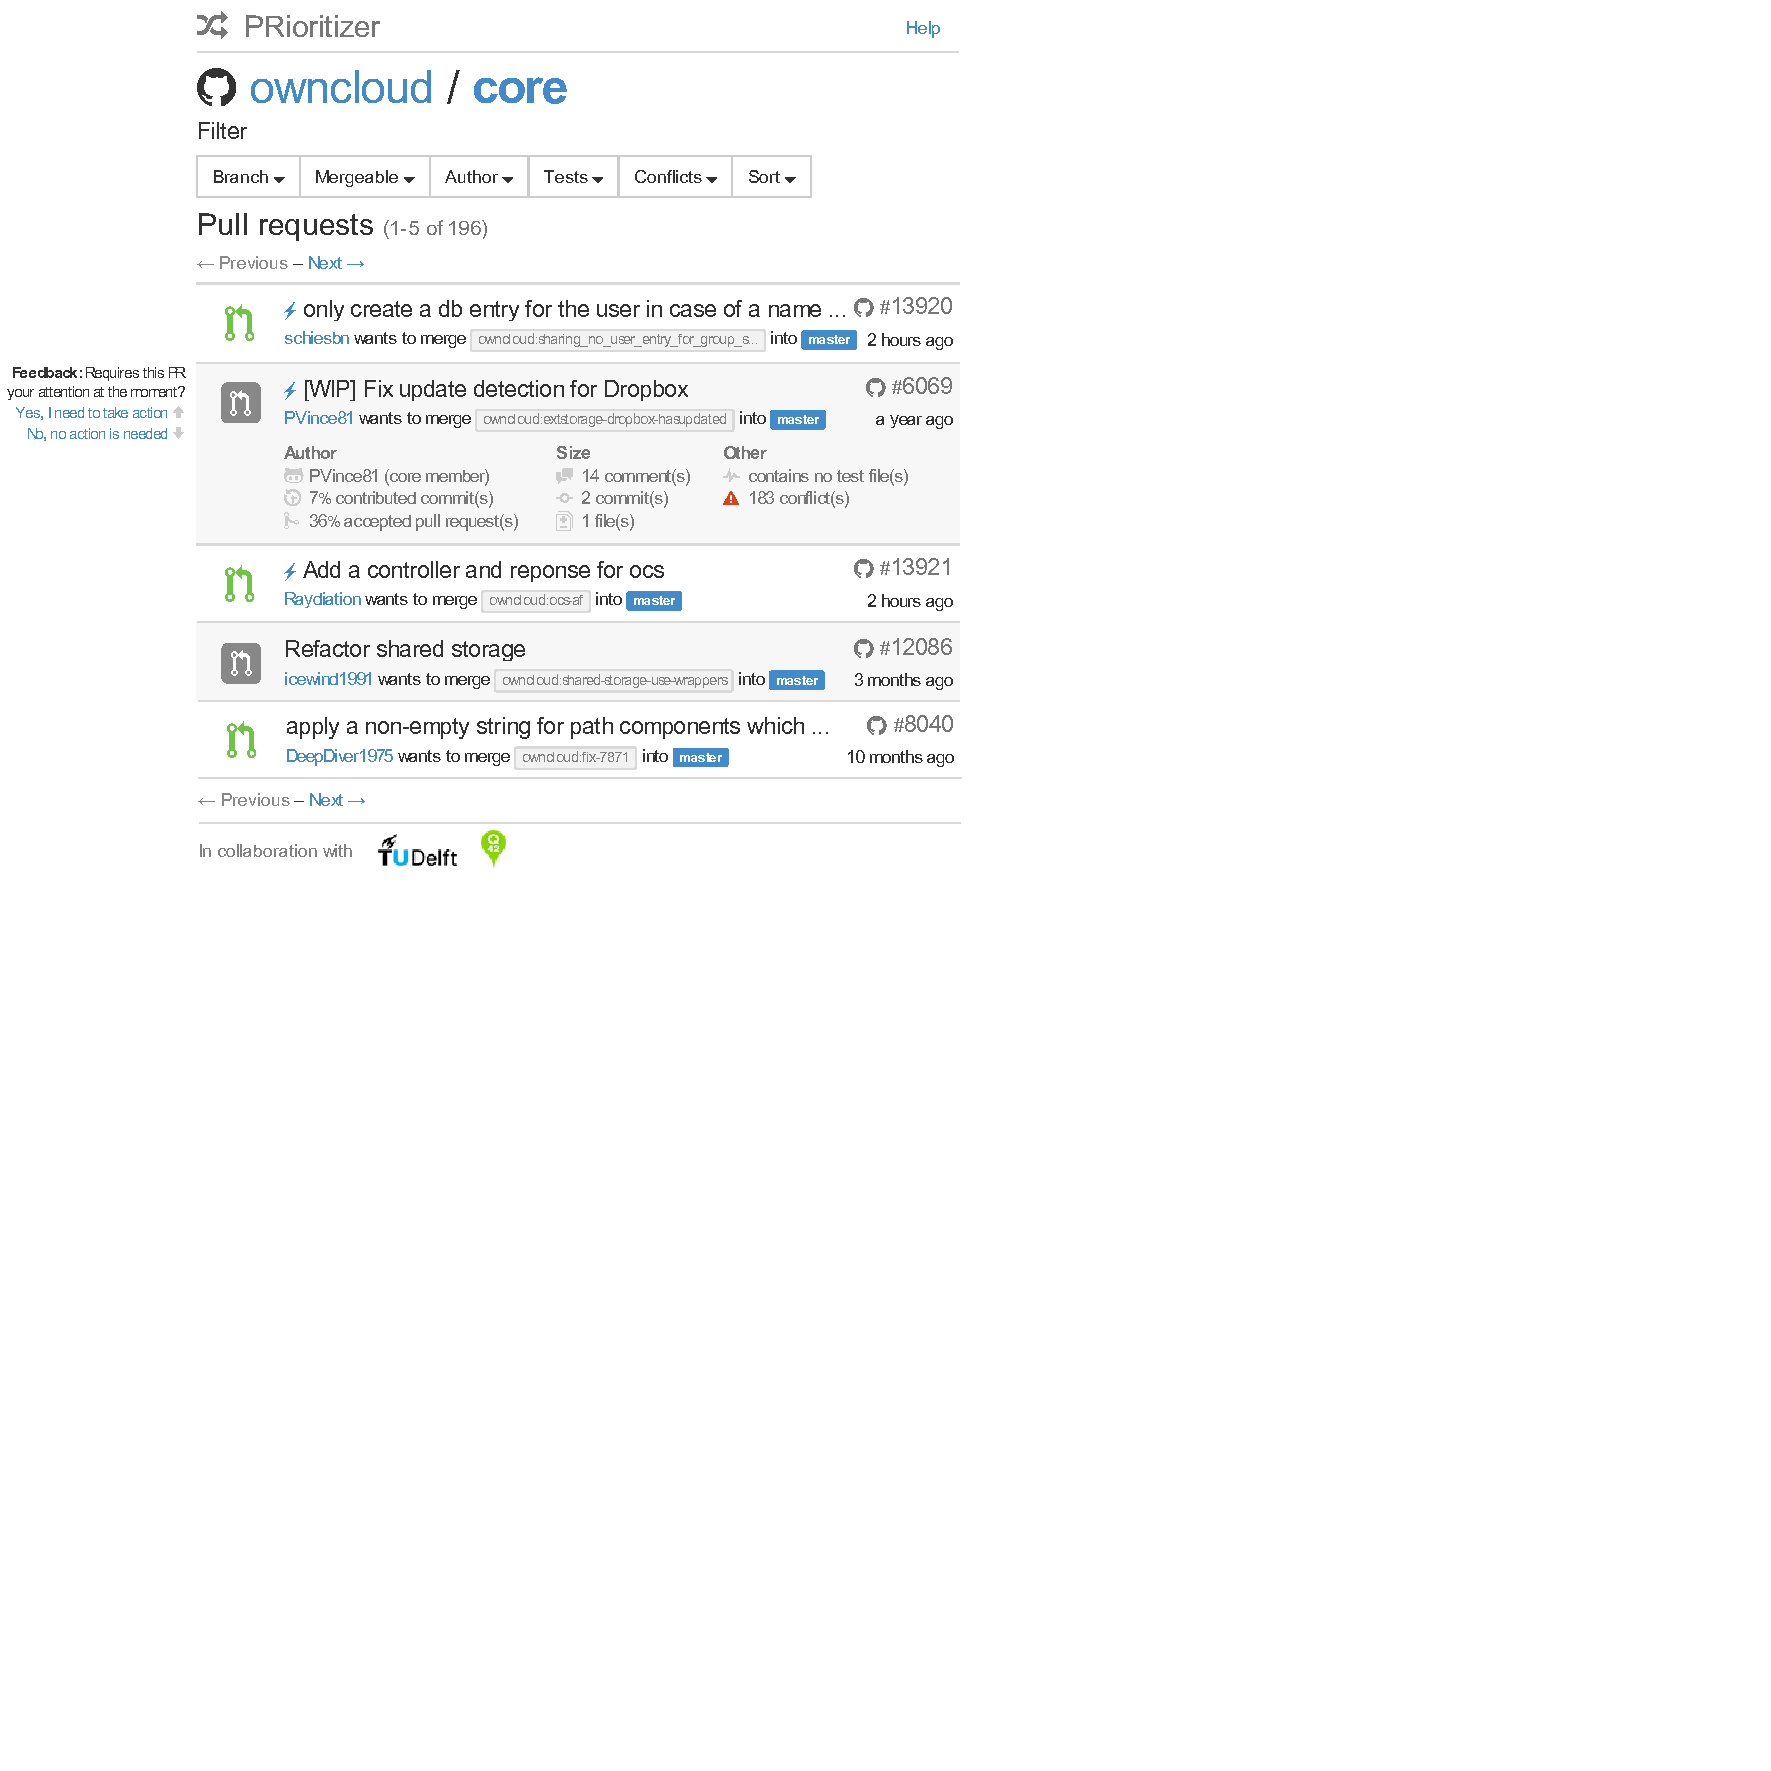
\includegraphics[width=0.5\textwidth]{../figs/interface.pdf}
  \caption[The user interface]
  {The user interface. It shows an ordered list of pull requests that need attention.}
  \label{fig:ui}
\end{figure}

\section{Initial Evaluation}
\label{sec:evaluation}

\subsection{How good are the activity predictions?}
\label{sec:learning}

To select an algorithm to base our prediction engine on, we used historical data
from 475 projects and three commonly used machine learning algorithms: Logistic
Regression, Na\"ive Bayes and Random Forests. The target of the test was to
compare how well models build with each algorithm could predict whether a pull
request would become active in the next time window against the ground truth
(what actually happened). We ran the three algorithms against each project with
a 10-fold random selection cross-validation. The models were trained with 90\%
training data and 10\% testing data.

The results show that both Logistic Regression and Na\"ive Bayes perform badly
on precision (0.36 and 0.34) and accuracy (0.62 and 0.60), which were our top
priorities. On the other hand, Random Forests perform better overall with a
precision of 0.64 and an accuracy of 0.85. To improve the performance, we tried
several optimisations like dataset balancing and feature pruning to no avail.

%\begin{table}
%  \begin{tabular}{lrrrrc}
%    \hline
%    \textbf{Algorithm} & \textbf{5\%} & \textbf{Mean} & \textbf{StDev} & \textbf{95\%} & \textbf{Histogram} \\
%    \hline
%
%    \bf{Logistic Regression}\\
%    Area Under Curve & 0.71 & 0.81 & 0.06 & 0.91 & 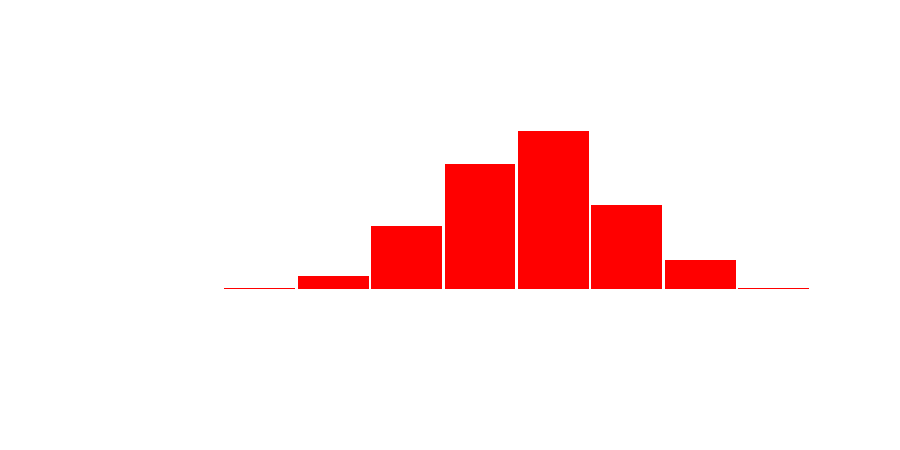
\includegraphics[scale = 0.09, clip = true, trim= 50px 60px 50px 60px]{../figs/hist-results/hist-LRauc.pdf} \\
%    Accuracy & 0.52 & 0.62 & 0.06 & 0.72 & 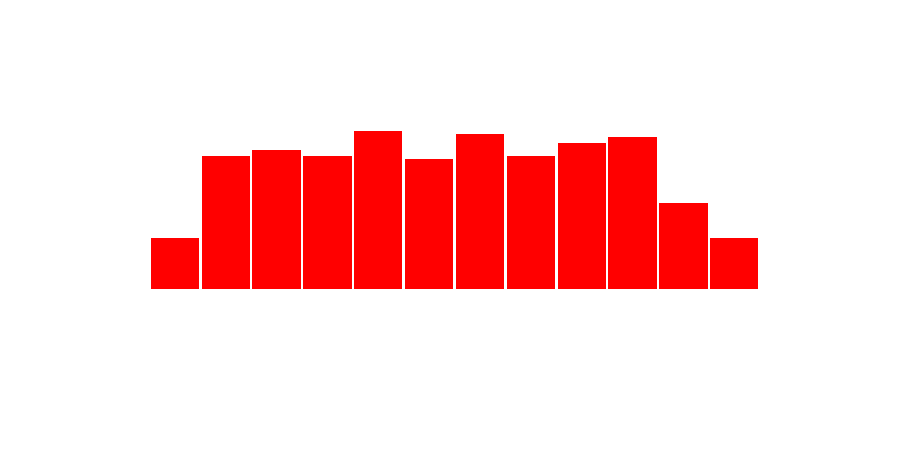
\includegraphics[scale = 0.09, clip = true, trim= 50px 60px 50px 60px]{../figs/hist-results/hist-LRacc.pdf} \\
%    Precision & 0.06 & 0.36 & 0.25 & 0.88 & 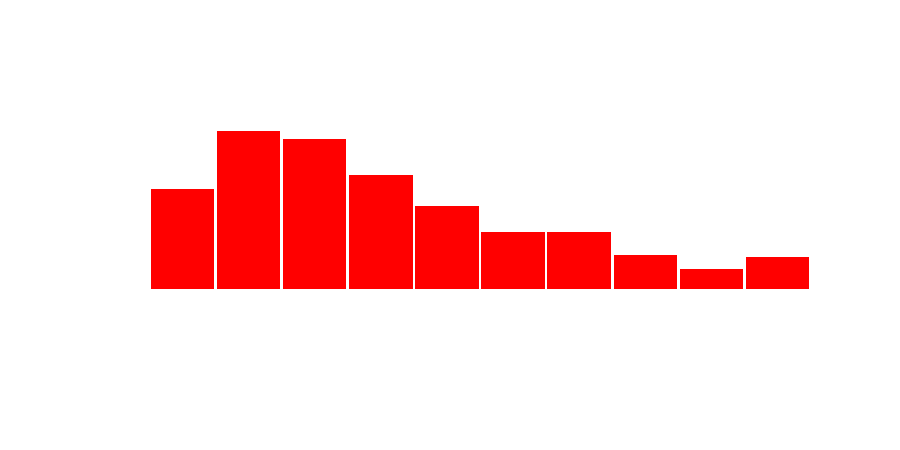
\includegraphics[scale = 0.09, clip = true, trim= 50px 60px 50px 60px]{../figs/hist-results/hist-LRprec.pdf} \\
%    Recall & 0.66 & 0.83 & 0.09 & 0.95 & 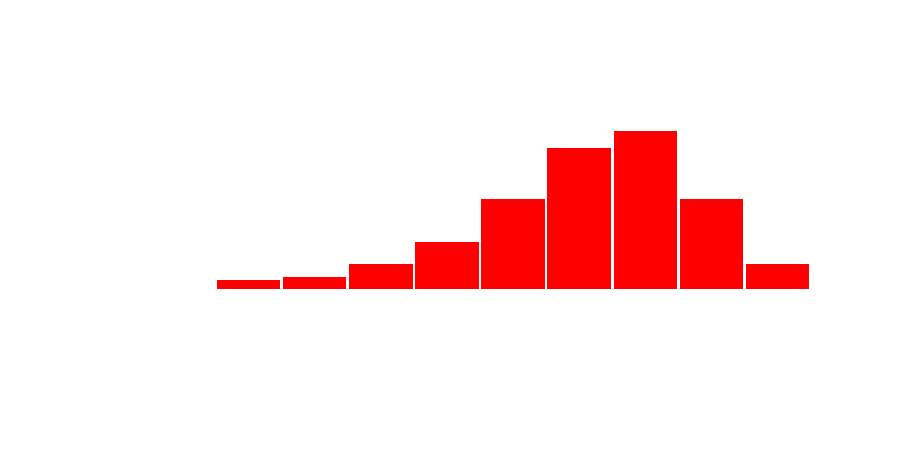
\includegraphics[scale = 0.09, clip = true, trim= 50px 60px 50px 60px]{../figs/hist-results/hist-LRrec.pdf} \\
%    F1 & 0.092 & 0.45 & 0.21 & 0.77 & 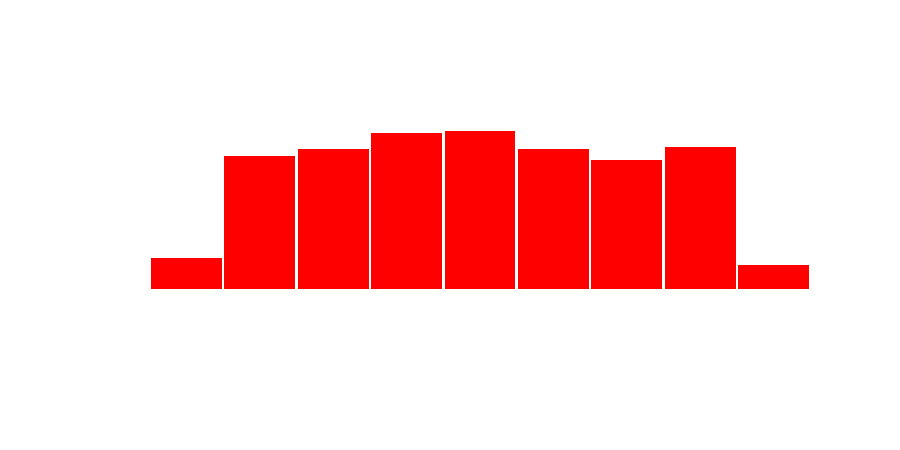
\includegraphics[scale = 0.1, clip = true, trim= 50px 60px 50px 60px]{../figs/hist-results/hist-LRf1.pdf} \\
%
%    \bf{Naive Bayes}\\
%    Area Under Curve & 0.65 & 0.75 & 0.06 & 0.86 & 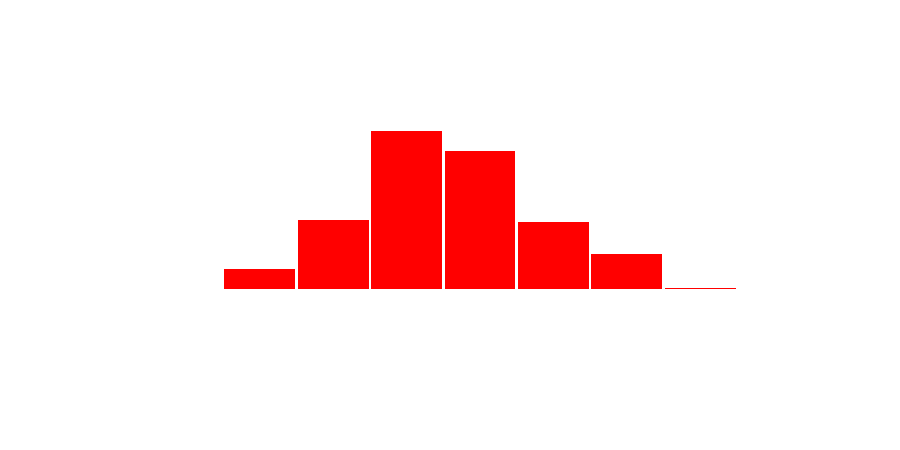
\includegraphics[scale = 0.09, clip = true, trim= 50px 60px 50px 60px]{../figs/hist-results/hist-NBauc.pdf} \\
%    Accuracy & 0.52 & 0.60 & 0.06 & 0.69 & 
\includegraphics[scale = 0.09, clip = true, trim= 50px 60px 50px 60px]{../figs/hist-results/hist-NBacc.pdf} \\
%    Precision & 0.06 & 0.34 & 0.23 & 0.82 & 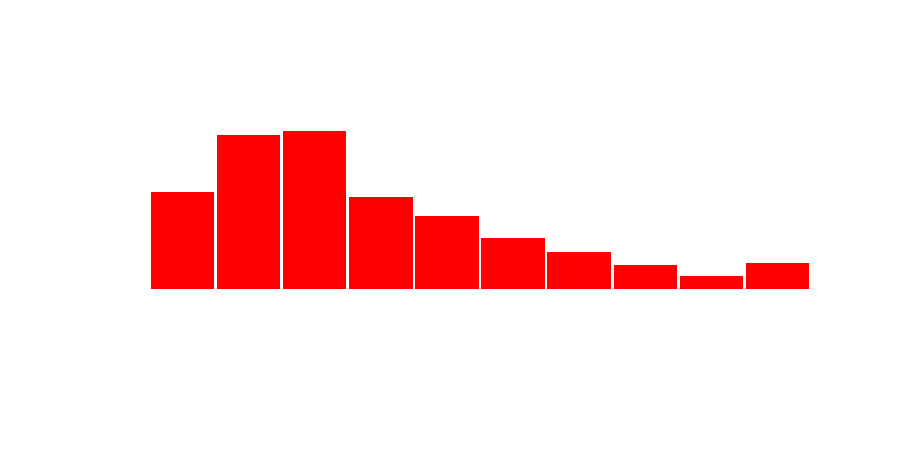
\includegraphics[scale = 0.09, clip = true, trim= 50px 60px 50px 60px]{../figs/hist-results/hist-NBprec.pdf} \\
%    Recall & 0.63 & 0.79 & 0.09 & 0.94 & 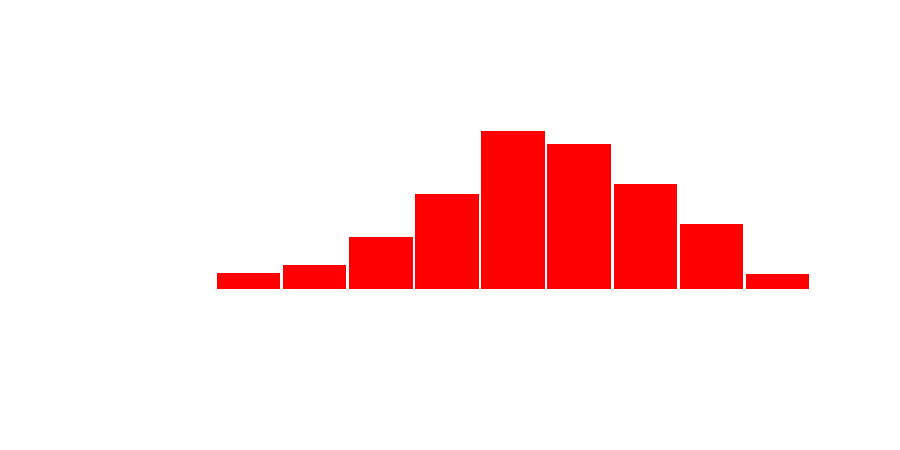
\includegraphics[scale = 0.09, clip = true, trim= 50px 60px 50px 60px]{../figs/hist-results/hist-NBrec.pdf} \\
%    F1 & 0.091 & 0.42 & 0.20 & 0.73 & 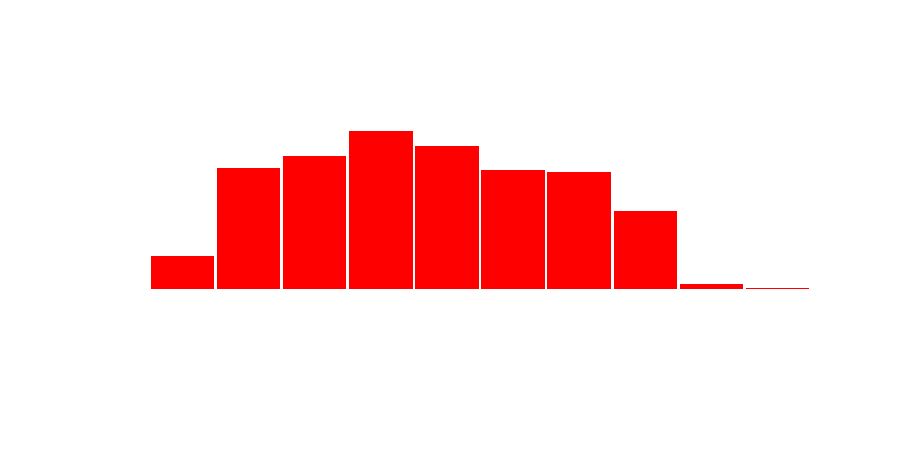
\includegraphics[scale = 0.1, clip = true, trim= 50px 60px 50px 60px]{../figs/hist-results/hist-NBf1.pdf} \\
%
%    \bf{Random Forest}\\
%    Area Under Curve & 0.81 & 0.89 & 0.05 & 0.95 & 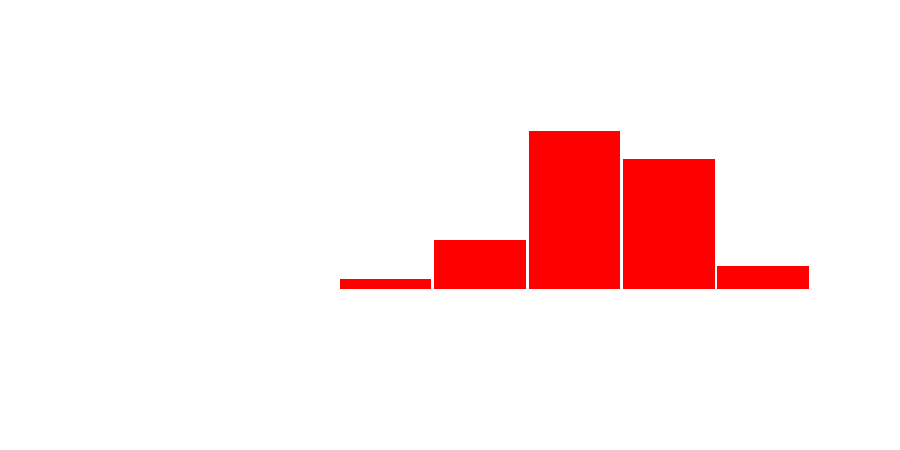
\includegraphics[scale = 0.09, clip = true, trim= 50px 60px 50px 60px]{../figs/hist-results/hist-RFauc.pdf} \\
%    Accuracy & 0.73 & 0.86 & 0.07 & 0.96 & 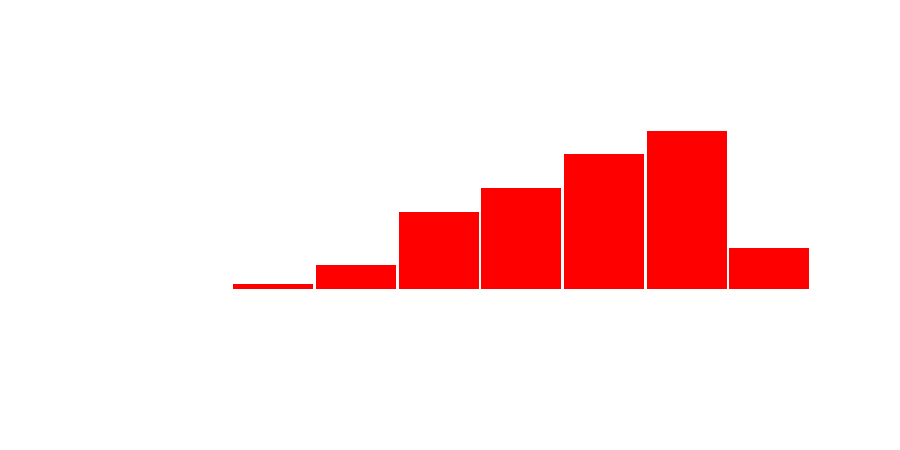
\includegraphics[scale = 0.09, clip = true, trim= 50px 60px 50px 60px]{../figs/hist-results/hist-RFacc.pdf} \\
%    Precision & 0.37 & 0.66 & 0.096 & 0.90 & 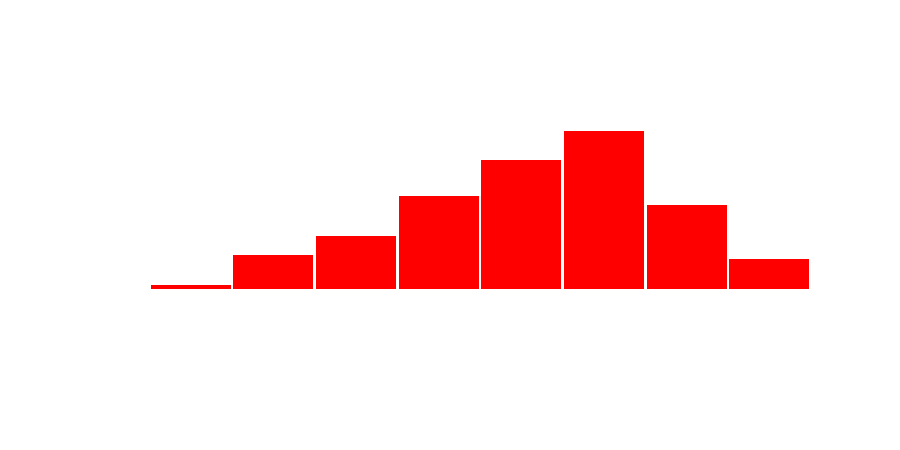
\includegraphics[scale = 0.1, clip = true, trim= 50px 60px 50px 60px]{../figs/hist-results/hist-RFprec.pdf} \\
%    Recall & 0.36 & 0.62 & 0.095 & 0.84 & 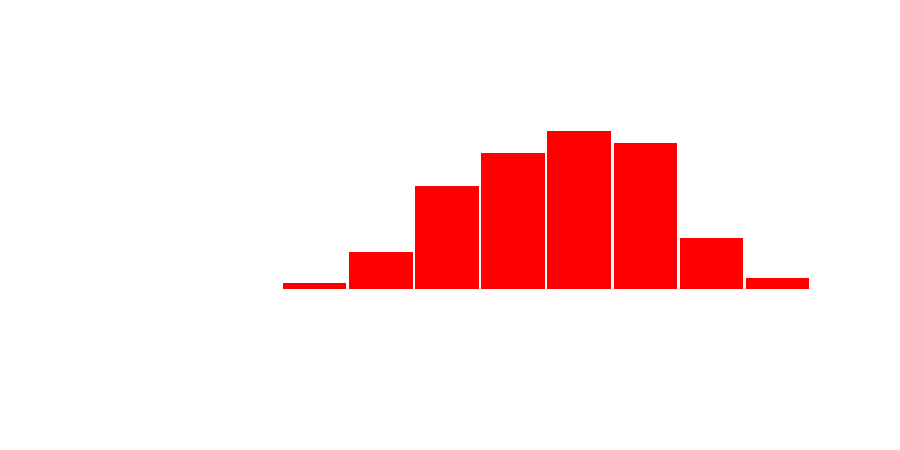
\includegraphics[scale = 0.1, clip = true, trim= 50px 60px 50px 60px]{../figs/hist-results/hist-RFrec.pdf} \\
%    F1 & 0.38 & 0.63 & 0.095 & 0.87 & 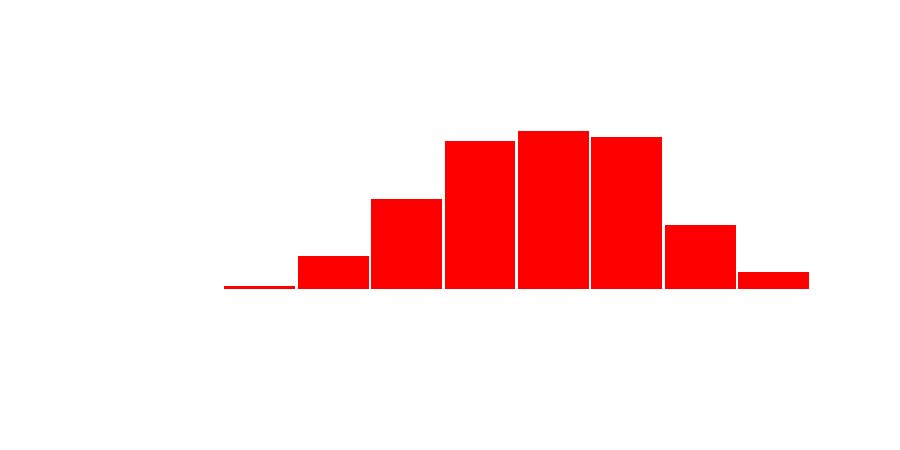
\includegraphics[scale = 0.1, clip = true, trim= 50px 60px 50px 60px]{../figs/hist-results/hist-RFf1.pdf} \\
%    \hline
%  \end{tabular}
%  \caption[Comparision of algorithms]{Scores and distributions of algorithm performance across projects.}
%  \label{tab:alg-compare}
%\end{table}

%It is interesting to see that the age is a very dominant factor when we look at
%the feature importance in figure~\ref{fig:feature-importance}.  This is probably
%the case because it is very likely that new pull requests receive comments
%within the first few days.  Since the age feature is so dominant it could impact
%the model in a bad way.  When we turned this particular feature off, the results
%were worse instead.  So it seems the age has a positive effect on the
%prediction.
%
%\begin{figure}
%  \centering
%  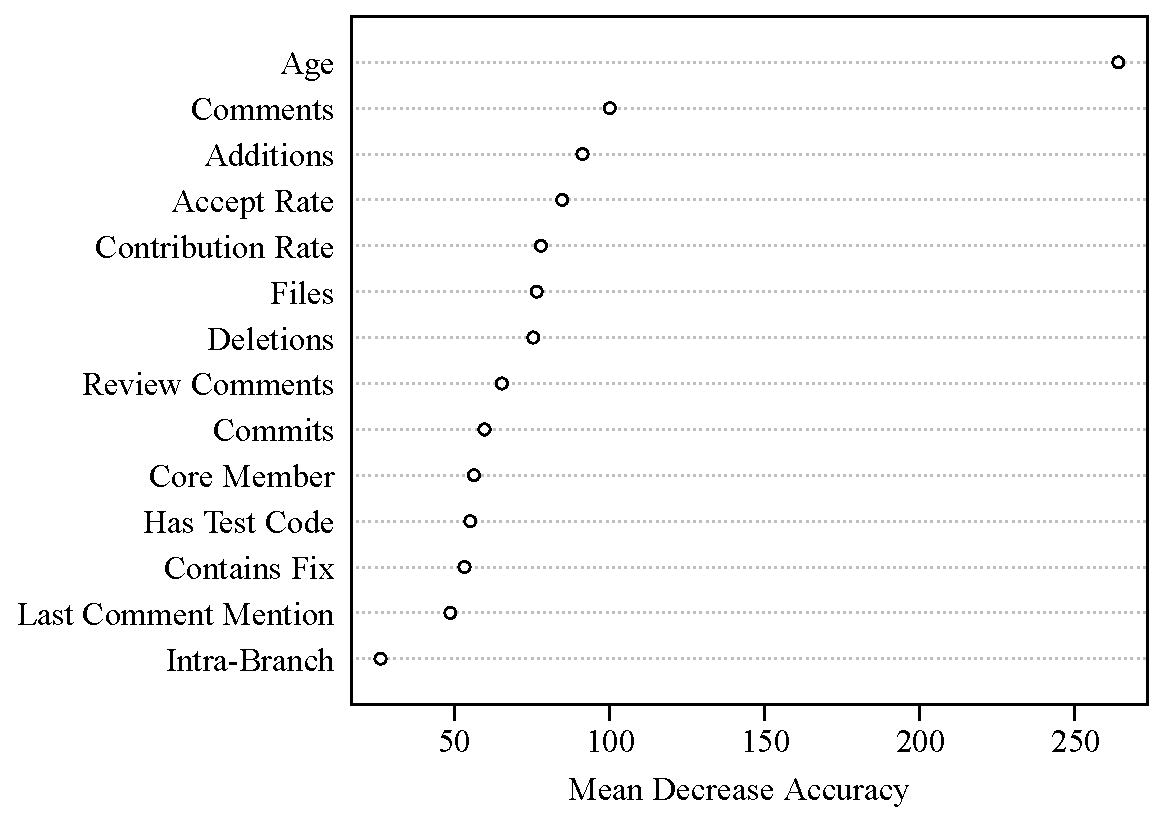
\includegraphics[width=0.45\textwidth]{../figs/mean-decrease-accuracy.pdf}
%  \caption[Plot of feature importance]
%   {Plot of feature importance of the aggregated projects. The age of the pull request is the dominant factor.}
%  \label{fig:feature-importance}
%\end{figure}

The results show that using Random Forests, we can predict with relatively high
accuracy (86\% on average across projects) whether a pull request in a given
time frame of its life will be active in the next one. This is an important
result for building a prioritizer service, as it gives us the confidence to
recommend a default ordering to the service user. Moreover, as the quality of
the prediction varies across projects, we can build preprocessing phases to
determine whether default recommendations can be useful.  However, there is room
for improvement: by selecting more representative features, or custom features
for each project, we can account for variations of pull request handling
practices. Moreover, user directed evaluation (already implemented in the
visualizer) can help retrofit our machine learning model with user preferences.

\begin{figure*}[t]
\centering
\subfigure {
  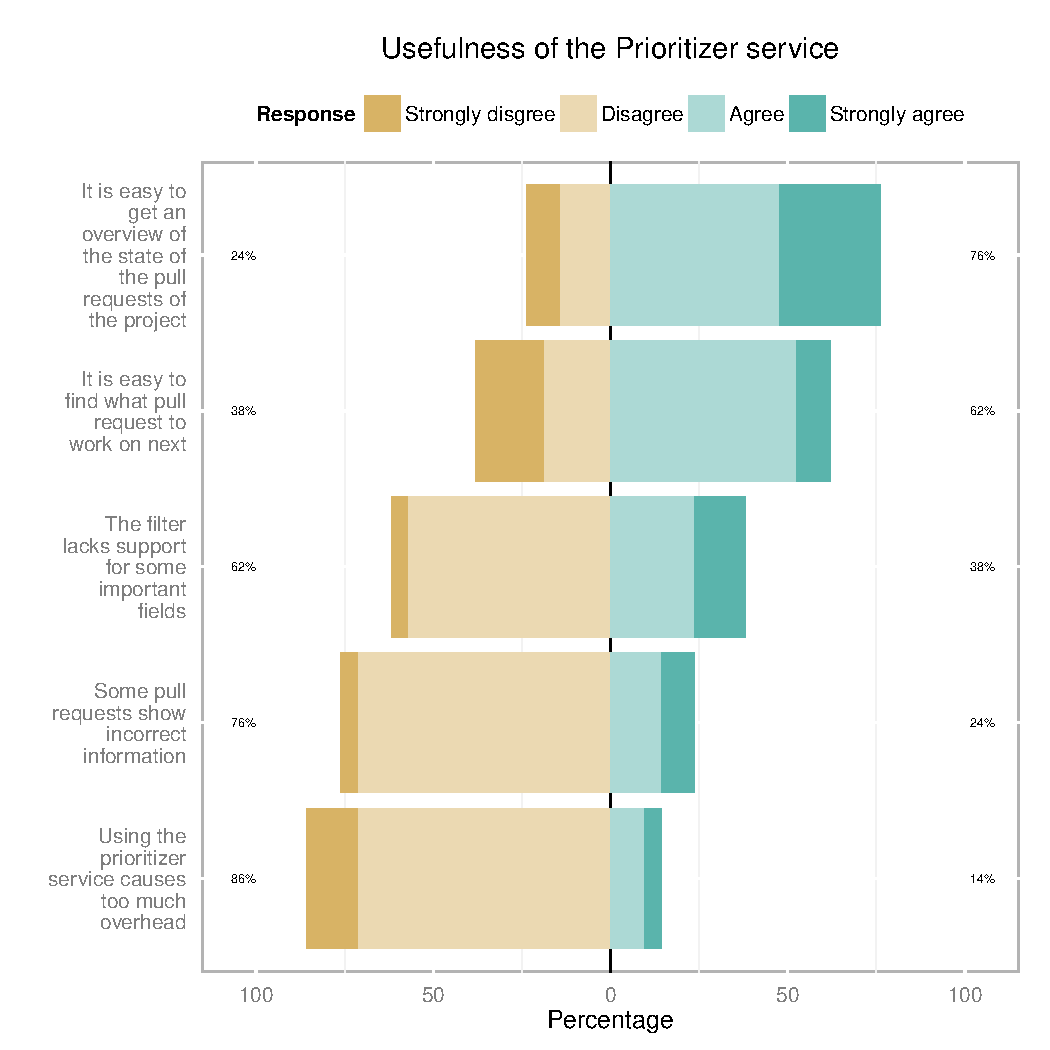
\includegraphics[scale=0.44]{../figs/service-userfulness.pdf}
  \label{fig:service-userfulness}
}
\subfigure{
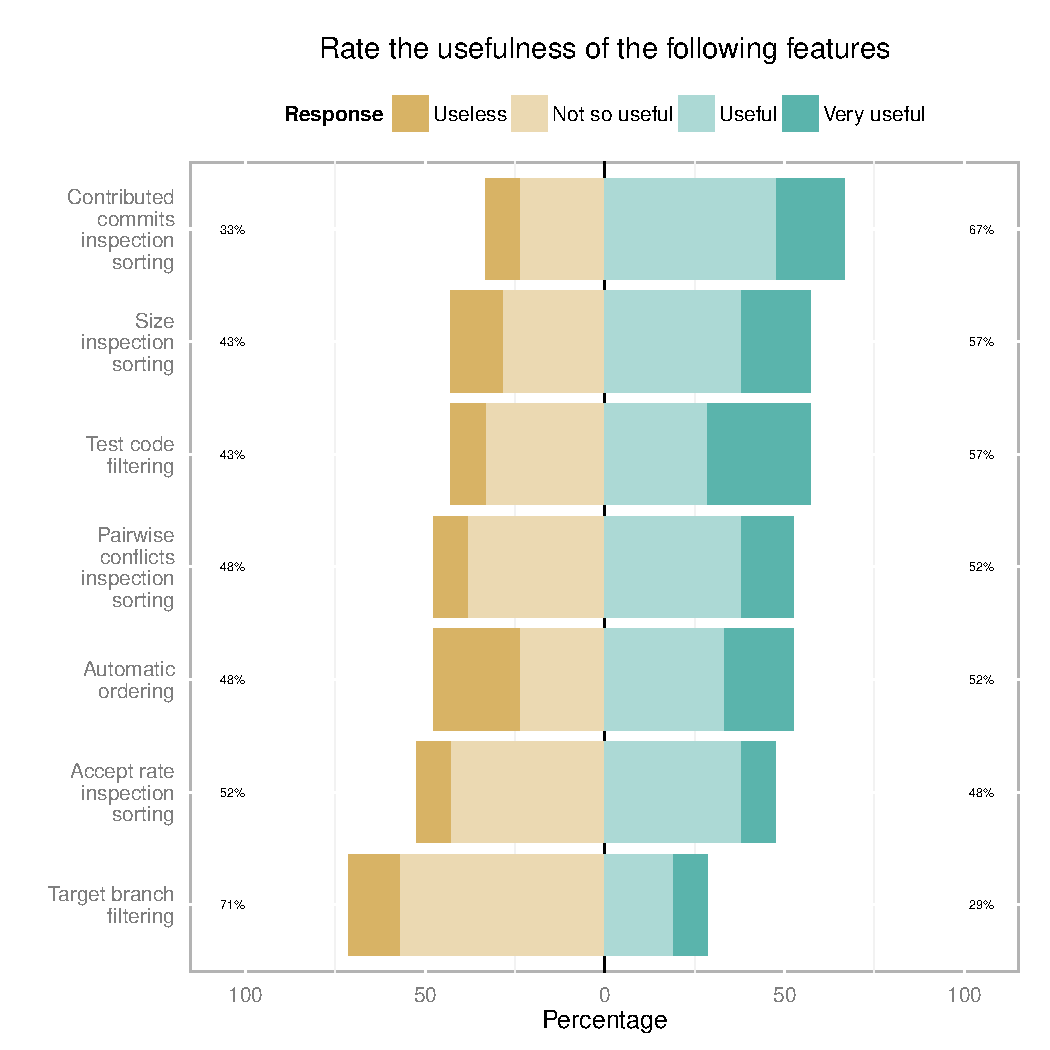
\includegraphics[scale=0.44]{../figs/feature-userfulness.pdf}
  \label{fig:service-userfulness}
}
\caption{User evaluation of the service and individual feature usefulness}
\label{fig:user-evaluation}
\end{figure*}

\subsection{Performance characteristics}

The \prioritizer runs incrementally on a set of pull requests. An initial import
involving training on a repository takes significantly longer than a normal run.
The time required to import ranges from a few minutes, for projects with less
than a hundred pull requests to a few hours for the biggest of projects. After
initial import, the prioritization time depends on the number of open pull
requests: for a medium sized project (30 open pull requests), the processing
takes less than a second, As a service, the \prioritizer is run on a machine
featuring a 3 GHz Quad core CPU and 16 GB of RAM. Without significant effort put
on performance optimization, it is capable of prioritizing 7 pull requests and
can simulate 400 pairwise merges per second.

\subsection{User Evaluation}

We performed a preliminary user evaluation in order to guide our future
developments of \prioritizer. For each of the 450 projects we used for
model building, we invited core team members of those projects to use it. The
invitation was sent by personal email containing a private link to the prioritizer
installation for their repository and a survey. The survey consisted of 4 odd
Likert-scale questions and 4 open ended ones. The Likert-scale questions invited
users to rate the usefulness of specific features and the overall service
quality while the open ended questions asked the users for missing features or
potential improvements. We received 21 answers.

Overall, as can be seen in Figure~\ref{fig:user-evaluation}, the usability of
\prioritizer has been positively perceived by human evaluators.  They
overwhelmingly state that \prioritizer would not cause extra overhead (86\%) and
that the \prioritizer interface can provide an easy to comprehend overview of
the overall project pull request status (76\%).  In the open ended responses,
the users indicated that pairwise conflict detection, target branches and the
pull request contributor profile were favourite features. As R1 states:
``\emph{I can see at a glance which PRs can be merged automatically. For some
reason the Github PR interface does not show this, you have to click on a PR to
find out if it can be automatically merged\ldots}''.

The main highlight of the service, automatic prioritization, received mixed
reviews; an equal number of people think that it is very useful and not useful at
the same time. From the open ended answers, we found that integrators do not
understand how automatic prioritization works. As
R17 puts it: ``\emph{It can show us the most pressing pull requests. However, it is unclear how this ranking is established, so I’d hope to know why a pull request is considered more urgent then others}''. As a consequence, 86\%
of the integrators mentioned that they would want more insight on how the automatic ordering works in future versions.

Finally we asked the respondents if they would use \prioritizer for their project. 57\% (12) of the respondent gave a positive answer.
We correlated the size of the project to the probability that integrators would
give a positive answer to the above question and found that integrators in
bigger projects tend to find prioritizer more useful
($\rho = 0.4307$).

\section{Related Work}

\section{Conclusions and Future Work}

\section*{Acknowledgements} The authors would like to thank Audris Mockus for
fruitful discussions that influenced the design of the prioritization algorithm.

\bibliographystyle{IEEEtran}
\bibliography{prioritizer}


\end{document}
